\chapter{The stemmatics of \mw{Buchedd Dewi}}
\label{cha:stemm-mwbuch-dewi}
The Welsh life of Saint David, known in Welsh as \mw{Buchedd Dewi} survives in several manuscripts from the fourteenth century onwards. 

Brynley Roberts states that the Latin \lat{Vita Davidis}, a late eleventh-century composition, was translated only in the late thirteenth century. He does not discuss at length why he dates the translation to this period, but he notes that the Welsh version derived from a later edition and omits certain practices and doctrinal elements~\autocite[218--219]{Rob_Ystoriaeu11}. \Textcite[lviii]{Eva_Welsh88}, however, dates the first Welsh translation to the early fourteenth century rather than the late thirteenth century.

I argue that the dating of this common exemplar may be done on linguistic grounds using my methodology of counting occurrences of lenition of voiceless stops. I also argue that statistical analysis of the orthography of voiceless stops may help in understanding the transmission and the stemmatics of thirteenth-century texts into the fourteenth century and beyond.



\section{The database}
\label{sec:database}

The database containing instances of lenition used here differs from that in the previous chapters. Here, only lenition of \mw[]{p, t, c} is counted, and research exceptions are not included or discussed even as research exceptions. Instances of free lenition, such as object lenition or adverbial phrase lenition, are only included if lenition is written for at least one mansucript.


More significantly, one entry does not consist of an instance where we would expect lenition in one manuscript text, but rather one instance in three manuscript texts, \gls{j119}, \gls{ll27}, and \gls{ctd22}. In this manner, it is possible to compare not only to what degree each manuscript represents lenition, but also which specific instances of lenition agree or disagree with one another between manuscripts. This way, it is possible to find out whether orthographical lenition was added in a common ancestral manuscript, or independently. Table~\ref{tab:samplebuchedddewi} provides a sample from the beginning of the database. Words are given in \gls{mow} orthography, because the exact spelling of these words may vary between manuscripts. The database contains 213 data points in total.

\begin{table}[h]\centering
% Table generated by Excel2LaTeX from sheet 'Sheet1'
\begin{tabular}{wlddcddcddc}
  \toprule
   & & \multicolumn{3}{c}{\gls{j119}} & \multicolumn{3}{c}{\gls{ll27}} & \multicolumn{3}{c}{\gls{ctd22}} \\
\tch{Word} & \tch{Cause lenition}  & \tch{f.} & \tch{l. } & \tch{len.} & \tch{f.} & \tch{l. } & \tch{len.} & \tch{f.} & \tch{l. } & \tch{len.} \\
\midrule
beisrudd & apposition & 93r & 3  & \FALSE & 62v & 24 & \TRUE & 138r & 3  & \TRUE \\
Grist & apposition & 93r & 7  & \TRUE & 62v & 27 & \TRUE & 138r & 7  & \TRUE \\
geffi & \mw{a} & 93r & 12 & \TRUE & 63r & 5  & \TRUE & 138r & 12 & \TRUE \\
ben & \mw{uch} & 93r & 14 & \TRUE & 63r & 6  & \FALSE & 138r & 14 & \FALSE \\
bieufydd & [\mw{a}] & 93r & 16 & \TRUE & 63r & 8  & \TRUE & 138r & 16 & \TRUE \\
Badrig & \mw{at} & 93r & 20 & \FALSE & 63r & 11 & \TRUE & 138v & 4  & \TRUE \\
garai & \mw{a} & 93v & 3  & \TRUE & 63r & 18 & \TRUE & 138v & 12 & \TRUE \\
Badrig & \ei & 93v & 3  & \FALSE & 63r & 18 & \TRUE & 138v & 12 & \TRUE \\
Badrig & fem.\ noun & 93v & 8  & \FALSE & 63r & 22 & \TRUE & 138v & 16 & \FALSE \\
beth & adv.\ phrase & 93v & 10 & \TRUE & 63r & 24 & \TRUE & 139r & 3  & \TRUE \\
gladdysid & \mw{a} & 93v & 13 & \TRUE & 63r & 27 & \TRUE & 139r & 6  & \TRUE \\
\bottomrule
\end{tabular}%


\caption{A sample from the database of lenition in \mw{Buchedd Dewi}.}
\label{tab:samplebuchedddewi}
\end{table}

\section{The manuscripts}
\label{sec:manuscripts-1}

The various manuscript in which \mw[]{Buchedd Dewi} survives are described by \textcite[lv--lviii]{Eva_Welsh88}. He notes that the text is extant in some fourteen manuscripts, and describes five of these. I have taken three of those five for analysis in this chapter.

\Acrlong{j119}, also called the Book of the Anchorite of Llanddewi Brefi dates to the mid-fourteenth century~\autocite{Tho_TEI13}. The manuscript's first text has a note in its preface. In this note, we find the manuscript was compiled for Gruffudd ap Llywelyn, who lived in northern Carmarthenshire. The note also contains a year, 1346, although it is quite certain to what it refers exactly. It might only have referred to when the first text was copied, and other texts may have been added later~\autocite[lvi--lvii]{Eva_Welsh88}.

\Acrlong{ll27}, also called the Red Book of Talgarth, dates to the turn of the fifteenth century. The manuscript was compiled for a nobleman called Hopcyn ap Thomas ab Einion of Ynystawe, north of Swansea~\autocite[lvii]{Eva_Welsh88}.

\Acrlong{ctd22} dates to the first half of the fifteenth century, not long after 1429~\autocite{Eva_Welsh88}. The writer of the manuscript is thought by \textcite[107]{Pow_description81} to be from South Wales. He based this on some dialectal forms found in the manuscript.

\subsection{The relationship between the manuscripts}
\label{sec:relat-betw-manuscr}
\textcite{Eva_Welsh88} discusses the relationship of the manuscripts:

\tqt{It appears that [\gls{ll27}] and [\gls{ctd22}] [\dots] derive originally from the same archetype, which is now lust, but which was different from [\gls{j119}]. That text and [\gls{j119}] must have come either directly or indirectly from the same text, which, however, could hardly have been the original copy. All extant copies have inherited errors made by an early copyist in an earlier text from which they all derive. This earlier text must have been itself a copy, made not long after the original composition of the work in the first half of the fourteenth century. It should be noted here that there are few serious textual divergences among the manuscripts.}{Eva_Welsh88}{lviii}

He posits a stemma for the extant manuscripts, which based on his wording above I reconstruct as in Figure~\ref{fig:stemmadewievans}.

\begin{figure}[h]
  \centering
  \begin{forest}
    where n children=0{tier=word}{}
    [α
    [\textit{β}
    [\gls{j119}]
    [γ[\gls{ll27}]
    [\gls{ctd22}]]]
    ]   
  \end{forest}
  \caption{Stemma of \mw[]{Buchedd Dewi} according to Evans.}
  \label{fig:stemmadewievans}
\end{figure}

\section{Some examples from \mw{Buchedd Dewi}}
\label{sec:some-examples-from}
Before showing the results, I list some examples that are not included in the databse because readings diverge too much between manuscripts to simply be counted as data points. Alternatively, they do not constitute lenition in the morphophonemic sense, but still show relevant orthographical variation. 
\begin{mwl}
  \mwc[ex:odalymj119]{\gls{j119} 93r.1}{Yma y treithir o ach deỽi ac o \al{dalym} o'e uuched}{Here the lineage of Dewi and part of his life are discussed.}
  \mwc[ex:odalymll27]{\gls{ll27} 62v.22}{val hynn y treythir o ach dewi ac o \al{beth} o'e vuched a'e wyrtheu}{Like this the lineage of Dewi and a part of his life and his miracles are discussed.}
  \mwc[ex:odalymctd22]{\gls{ctd22} 138r.1}{yma y treithir o ach dewi ac o \al{dalym} oe vuched}{Here the lineage of Dewi and a part of his life are discussed.}
\end{mwl}
Here, we see both \mw[part]{dalym} and \mw[thing]{beth} used. Both of these words start with a voiceless stop in their radical form, but they are different words. It is not obvious which one is the original reading, and it is therefore impossible to say which of these readings are orthographical updates to an original \mw[]{t} or \mw[]{p}, and which readings are later additions.

\begin{mwl}
  \mwc[ex:ogaryatj119]{\gls{j119} 93v.9--10}{A thra diodeuy laỽer \al{o garyat} duỽ}{And although you allow much love of God.}
  \mwc[ex:ogaryatll27]{\gls{ll27} 63r.23}{a thi a odefy lawer yno \al{yr kareat} ar duỽ}{And there you allow much love of God.}
  \mwc[ex:ogaryatctd22]{\gls{ctd22} 139r.1--2}{a thi a diodefy lawer yno \al{yr karyat} duỽ}{And there you allow much love of God.}
\end{mwl}
Here, \gls{j119}'s \mw[out of love]{o garyat} is not matched by the same construction in the other manuscripts. In the other manuscripts, this word does not stand in a position that would cause it to be lenited. Again, it is difficult to say which of these readings is the original one.

\begin{mwl}
  \mwc[ex:dosdij119]{\gls{j119} 94r.9}{dos \al{ti} heb y sant}{``Come,'' said the saint}
  \mwc[ex:dosdill27]{\gls{ll27} 63v.16--17}{Dos \al{di} heb y sant}{``Come,'' said the saint}
  \mwc[ex:dosdictd22]{\gls{ctd22} 139v.10--11}{Dos \al{di} heb y sant}{``Come,'' said the saint}
\end{mwl}
Lenition in \mw[you]{ti/di} is optional here, as lenition does not impinge on grammaticality or meaning in any way. It is an instance of petrification. Still, the contrast between unlenited and lenited forms provides evidence that scribes changed the orthography between \mw[]{t} and \mw[]{d}, even if this specific example does not tell us which one is the original.

\begin{mwl}
  \mwc[ex:ysgotj119]{\gls{j119} 95v.20--21}{Ac yna yd argannuv tyỽyssaỽc a elỽit boya. Ac \al{yscot} oed y mỽc hỽnnỽ}{And then the prince who was called Boya, and he was a Irishman, discovered that smoke.}
  \mwc[ex:ysgotll27]{\gls{ll27} 65r.8--9}{Ac yna yd arganvu tywyssaỽc a elwit boya \al{o gysgot} y mỽc hỽnnỽ}{And then the prince who was called Boya from shadow discovered that smoke.}
  \mwc[ex:ysgotctd22]{\gls{ctd22}142r--142v.15--1}{ac yna yd arganuu tywyssaỽc a elwit boya ac \al{yscott} oed.\ y niver hỽnnỽ}{And then the prince who was called Boya, and he was a Irishman, discovered that number.}
\end{mwl}
Here, we find both \mw[Irishman]{yscot} and \mw[from shadow]{o gysgod}. The former reading is the uncorrupted one, as the Latin has \lat{Scottus}~\autocite[155]{Wad_Vitae13}.

\begin{mwl}
  \mwc[ex:wdostij119]{\gls{j119} 97v.1--2}{Tidi ỽrda gỽnuydedic pony \al{ỽdosti} heb ef}{``You, blessed nobleman, do you not know?'', said he.}
  \mwc[ex:wdostill27]{\gls{ll27} 66r.24}{Tydi wr da gỽynuydedic pony wdost \al{di} heb ef}{``You, blessed nobleman, do you not know?'', said he.}
  \mwc[ex:wdostictd22]{\gls{ctd22} 145r.3--4}{Tydi wrda gỽynuededic pony wdost \al{ti} heb ef}{``You, blessed nobleman, do you not know?'', said he.}
\end{mwl}
This example shows grammatically and semantically trivial variation between \mw[you]{ti} and \mw[]{di}, and is exactly equivalent to Examples~\ref{ex:dosdij119}, \ref{ex:dosdill27}, and \ref{ex:dosdictd22}.

\begin{mwl}
  \mwc[ex:eistebawpj119]{\gls{j119} 98r.9}{A gỽedy eiste \al{paỽb} yn y mod y dylyynt}{And after everybody sitting in the way they ought to}
  \mwc[ex:eistebawpll27]{\gls{ll27} 66v.24}{A gỽedy eisted \al{o baỽp} yn y mod y dylyynt}{And after everybody sitting in the way they ought to}
  \mwc[ex:eistebawpctd22]{\gls{ctd22} 146r.4--5}{a gỽedy eisted \al{o baỽp} yn y mod y dylyynt}{And after everybody sitting in the way they ought to}
\end{mwl}
Both readings --- \mw[everyone sitting]{eiste paỽb, eisted o baỽp} --- are equally valid, but lenition is only expected in the latter reading. It is therefore impossible to say whether expected lenition is represented in all cases, because it is not expected in all readings.

\begin{mwl}
  \mwc[ex:aeprouassamj119]{\gls{j119} 99r.2--3}{A ni \al{a'e prouassam} pob eilỽers.}{And we proved it one by one.}
  \mwc[ex:aeprouassamll27]{\gls{ll27} 67v.7}{a ni \al{a'e profassam} bob eilwers.}{And we proved it one by one.}
  \mwc[ex:aeprouassamctd22]{\gls{ctd22} 147v.3}{a ni \al{a prouassam} bob eilwers.}{And we proved one by one.}
\end{mwl}
It is unclear here whether the infixed object particle \mw[him]{'e} is added to account for lack of lenition in Examples~\ref{ex:aeprouassamj119} and \ref{ex:aeprouassamll27}, or alternatively lack of lenition in \ref{ex:aeprouassamctd22} is due to the deletion of the object particle. Because two readings are reconstructable, the example cannot be counted.

\begin{mwl}
  \mwc[ex:trydedweithj119]{\gls{j119} 99v.6}{a rodes \al{tryded} ỽeith o gyduundeb yr holl seint}{And he gave a third time of agreement of all the saints.}
  \mwc[ex:trydedweithll27]{\gls{ll27} 68r.4--5}{Ar \al{dryded} weith o gytuundeb yr hoỻ seint}{And the third time of agreement of all the saints.}
  \mwc[ex:trydedweithctd22]{\gls{ctd22} 148v.2--3}{ar \al{dryded} weith o gyttundeb yr holl seint}{And the third time of agreement of all the saints.}
\end{mwl}
Here, \mw[third]{tryded} is found in leniting position in \gls{ll27} and \gls{ctd22}, but not in \gls{j119}.

\begin{mwl}
  \mwc[]{\gls{j119} 100v.13--14}{gann dyrchauel ohonaỽ y benn brynn vchel y lle y buassei bregeth \al{kynn} o hynny}{by his rising to the top of the high hill, the place where a sermon had been before that.}
  \mwc[]{\gls{ll27} 68v.22--23}{gan dyrchafel ohonaỽ y benn brynn uchel.\ y lle y buassei bregeth \al{kynn} no hynny.}{by his rising to the top of the high hill, the place where a sermon had been before that.}
  \mwc[]{\gls{ctd22} 150r.11--12}{gan drychafel ohanaỽ y ben bryn uchel.\ y lle y buassei pregeth \al{gyn} no hynny}{by his rising to the top of the high hill, the place where ha sermon had been before that.}
\end{mwl}
Here, we see \mw[before]{gyn} being lenited in \gls{ctd22}. This lenition could be thought of as an instance of adverb lenition, because \mw[before that]{gyn no hynny} is an adverbial phrase to the verb. However, \mw[before]{gyn} is not typically lenited in this position in \gls{mw} or even \gls{mow}. 

\begin{mwl}
  \mwc[ex:yngynj119]{\gls{j119} 100v.24}{ac yn \al{gynn gyffredinet}}{And as common as}
  \mwc[ex:yngynll27]{\gls{ll27} 69r.5}{ac yn \al{gyffredinet}}{And [as] common as}
  \mwc[ex:yngynctd22]{\gls{ctd22} 150v.6}{ac yn \al{gyn gyffredinet}}{And as common as}
\end{mwl}
The word \mw[]{gyn} is erroneously removed in \gls{ll27}. The sentence is ungrammatical without it, so its removal is a scribal error. Still, we cannot know now whether \gls{ll27} would have had \mw[]{cyn} or \mw[]{gyn} otherwise, so this instance cannot be counted.

\begin{mwl}
  \mwc[ex:thangneuedj119]{\gls{j119} 101v.23}{arglỽyd kymer dy ỽas \al{y'thangneued}.}{Lord, take your servant to your peace.}
  \mwc[ex:thangneuedll27]{\gls{ll27} 69v.19--20}{arglỽyd kymer dy was \al{y'th dangnefed}.}{Lord, take your servant to your peace.}
  \mwc[ex:thangneuedctd22]{\gls{ctd22} 152r.10}{arglỽyd kymer di dy was \al{y'th dagneued}.}{Lord, take your servant to your peace.}
\end{mwl}
Here, Example~\ref{ex:thangneuedj119} from \gls{j119} has \mw[]{y thangneued} for \mw[your peace]{y'th dangneued}. Perhaps the scribe of \gls{j119} erroneously interpreted the expression as `her peace', which does not make sense in context. This does beg the question what sort of exemplar would invite such an erroneous reading. Hypothetical \mw[]{tht} in *\mw[]{ythtangneued} could perhaps be mistaken for an archaic spelling of /θ/. If so, this example is evidence that \gls{j119}'s exemplar did not have orthographic lenition here.

\begin{mwl}
  \mwc[]{\gls{j119} 102v.1--2}{Yna y gỽelut ti \al{gyfuredec} gann seint yr ynys honn.}{}
  \mwc[]{\gls{ll27} 70r.19--20}{Yna y gỽelit \al{kyfredec} gan seint yr ynys honn.}{\todo{This one might be hypercorrect lenition in j119, and the proper reading might be CTD22: \mw{ymgyfredec}. Impersonal forms usually never cause object lenition~\autocite{vanSluisdevelopmentpostverballenition2014}.}}
  \mwc[]{\gls{ctd22} 153r.10--11}{yna y gỽelit \al{ymgyfredec} gan seint yr enys hon.}{}
\end{mwl}

\begin{mwl}
  \mwc[ex:missingsj119]{\gls{j119} 102v.21--22}{A gỽedy daruot idaỽ rodi y venndith y baỽp.}{And after it happened to him that he gave his blessing to everyone.}
  \mwc[ex:missingsctd22]{\gls{ctd22} 154r.1--3}{A gwedy daruot ydaỽ rodi y vendith y baỽp}{And after it happened to him that he gave his blessing to everyone.}
\end{mwl}

The whole sentence found in Examples~\ref{ex:missingsj119} and~\ref{ex:missingsctd22} is missing in \gls{ll27}.

\section{Results}
\label{sec:results-1}
As can be seen in Table~\ref{tab:replendewi}, lenition of \mw[]{c} is represented in nearly all instances. The other consonants are represented less regularly.
\begin{table}[h]
\centering
\begin{tabular}{lddd}
\toprule
     \tch{MS}         & \tch{\mw{p}}      & \tch{\mw{t}}      & \tch{\mw{c}}       \\ \midrule
\gls{j119}  & 67.5 & 65.9 & 99.0  \\
\gls{ll27}  & 88.3 & 85.4 & 97.9  \\
\gls{ctd22} & 79.2 & 90.2 & 100.0 \\ \bottomrule
\end{tabular}
\caption{Percentual representation of lenition of voiceless stops in three versions of \mw[]{Buchedd Dewi}}
\label{tab:replendewi}
\end{table}

  \begin{figure}[h]
    \centering
    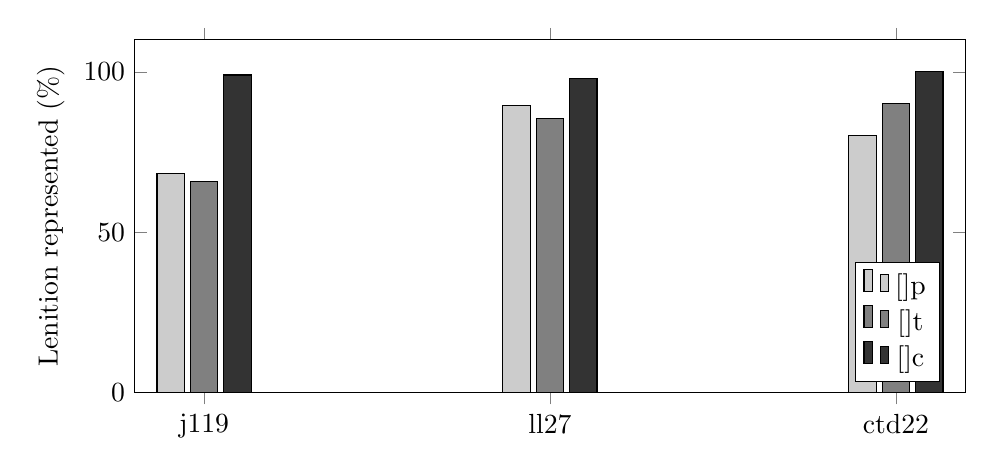
\begin{tikzpicture}
      \begin{axis}[
        ybar,
        ymin=0,
        width=\linewidth,
        height=.5\linewidth,
        % xlabel=Manuscript,
        ylabel={Lenition represented (\%)},
        legend pos = south east,
        symbolic x coords={
          \gls{j119},\gls{ll27},\gls{ctd22}},
        xtick=data,
        ]
        \addplot [fill=black!20] coordinates {
          (\gls{j119}, 68.42)
          (\gls{ll27}, 89.47)
          (\gls{ctd22},80.26)
        };
        \addplot [fill=black!50] coordinates{
          (\gls{j119}, 65.85)
          (\gls{ll27}, 85.37)
          (\gls{ctd22},90.24)
        };
        \addplot [fill=black!80] coordinates{
          (\gls{j119}, 99.00)
          (\gls{ll27}, 97.92)
          (\gls{ctd22},100.00)
        };
        \legend{\mw[]{p},\mw[]{t},\mw[]{c}}
      \end{axis}
    \end{tikzpicture}
    \caption{Percentual representation of lenition of voiceless stops in the various recensions of \mw[]{Buchedd Dewi}.}
    \label{fig:barchartdewi}
  \end{figure}


Non-representation of lenited \mw[]{c} is found in three instances. In all three instances, we are dealing with free lenition, which tends to be applied inconsistently in Middle Welsh:


The consistency with which lenition of \mw[]{c} is written implies that the Welsh exemplar was written at a time when lenited \mw[]{c} was already written with \mw[]{g}. This pattern of writing lenition of \mw[]{c}, but not \mw[]{p, t} is found from the second half of the thirteenth century onwards. This is evidence that \textcite{Rob_Ystoriaeu11} was right in positing the late thirteenth century as the time when the Welsh translation was composed.

Lenition of the remaining two consonants, \mw[]{p, t}, is written inconsistently. For these consonants, there are two possible scenarios: either lenition is added independently in each of the three manuscripts, or it is added in a common exemplar and then copied by two or three of these manuscripts. Quantitative methods may help in deciding between each of these scenarios.


\section{A statistical excursus}
\label{sec:statistical-excursus}


Chapter~\todo{laws}\ref{cha:welsh-laws} shows that texts originally composed in the thirteenth century and then copied in the fourteenth century replace \mw{p, t, c} for lenited voiceless stops with \mw{b, d, g}, but that they never do so completely. Chapter~\todo{brut}\ref{cha:indep-comp-mwbr} shows that original texts composed from the fourteenth century onwards do write lenited voiceless stops with \mw{b, d, g} consistently.

Taking the insights from these two chapters together, we are able to test whether a Welsh text found in the fourteenth century or later has a Welsh-language ancestor from the thirteenth century or earlier. If lenition of voiceless stops is represented haphazardly, this is evidence it dates from before the fourteenth century. Subfigure~\ref{sfig:pre1250} illustrates this scenario. If lenition of voiceless stops is written consistently, then there is no evidence of a pre-fourteenth-century composition. Subfigure~\ref{sfig:post1250} illustrates this scenario.

It is also possible to diagnose whether two exemplars of a text originally composed in the thirteenth century or earlier have a shared common ancestor from after the thirteenth century. Subfigure~\ref{sfig:intermediate} illustrates this scenario. If we hypothesise that two texts have a stemma of the type found in Subfigure~\ref{sfig:intermediate}, we would expect partial orthographic lenition of voiceless stops in both manuscripts, but the specific instances of lenition or lack thereof would agree with each other in more instances than what would be expected from chance.

\begin{figure}[h]
  \centering
  \subfloat[]{
    \label{sfig:pre1250}
    \begin{forest}
      [μ < 1250
      [X > 1300]
      [Y > 1300]]
    \end{forest}}
  \subfloat[]{
    \label{sfig:post1250}
    \begin{forest}
      [μ > 1300
      [X > 1300]
      [Y > 1300]]
    \end{forest}}
    \subfloat[]{
    \label{sfig:intermediate}
    \begin{forest}
      [μ < 1250
      [ν > 1300
      [X > 1300]
      [Y > 1300]]]
    \end{forest}}
  \caption{Hypothetically reconstructable stemmata based on the orthography of lenited voiceless stops.}
  \label{fig:possiblestemmata}
\end{figure}

The scenario of Subfigure~\ref{sfig:post1250} is easy to differentiate from the scenarios of Subfigure~\ref{sfig:pre1250} and Subfigure~\ref{sfig:intermediate}: the only thing one would have to check is whether lenition of voiceless stops is represented consistently. It is harder to differentiate between the remaining two scenarios. In the scenario of Subfigure~\ref{sfig:pre1250}, haphazard lenition would be found in both surviving manuscripts, but lenition or lack thereof would not correspond to one another to a degree beyond what would be predicted by chance. In order to argue for the scenario of Subfigure~\ref{sfig:intermediate}, one would have to demonstrate that the orthography of lenited voiceless stops agrees in so many specific instances that the partial addition of orthographically lenited voiceless stops is unlikely to be due to chance.

We can only say that a pattern is unlikely to be due to chance if we actually know what chance looks like. It is therefore necessary to form a picture of what chance would look like. The expected percentage of instances agreeing between manuscripts X and Y would be calculated as follows:
\[P(\text{X} = \text{Y}) = (P(\text{X}) \cap P(\text{Y})) + (P(\text{X}^C) \cap P(\text{Y}^C))\]
Here, \(P\) stands for the probability of the event in brackets following it.  \(P(\text{X})\) stands for the rate by which lenition is added in manuscript X, and \(P(\text{Y})\) means the same thing for manuscript Y. The sign \(\cap\) stands for the intersection of two probabilities, in this case the probability of both X and Y causing lenition. The \(^C\) stands for the complement of a probability, \ie the probability of something not happening. So, the equation above may be phrased as: the probability of X and Y independently agreeing on orthographical lenition is equal to the product of their respective probabilities of adding lenition plus the product of their respective probabilities of not adding lenition.

To make this formula more concrete, let's assume manuscript X adds orthographical lenition in 60\% of its instances, and manuscript Y adds orthographical lenition in 30\% of its instances. X and Y do not share a common ancestor that postdates orthographical lenition. In this case, the expected probability of X and Y agreeing on the orthography of lenition in a specific instance would be:

\[(0.6 \times 0.3) + (0.4 \times 0.7) = 0.18 + 0.28 = 0.46\]

So, any instance of a lenited voiceless stop would have an 18\% probability of being orthographically represented in both manuscripts by coincidence, and would have a 28\% probability of not being represented in both manuscripts. They would thus have a probability of 46\% of agreeing. A corpus of 100 instances of lenition of voiceless stops would be expected find 46 in agreement, and 54 in disagreement.

What kind of patterns should we ascribe to common inheritance of orthographical lenition? First of all, chance can be the cause of every single pattern, so it is never impossible to exclude coincidence as the cause for a group of extremely similar looking manuscripts. We can merely reject chance as a factor because it is \emph{unlikely} to have been the cause of a particular pattern, not because it is \emph{impossible}.

Sciences employing quantitative methods typically reject the null hypothesis if a correlation at least as strong as the observed results has a lower than one in twenty probability of being observed due to chance.  The null hypothesis is the hypothesis that there is no relationship between two measured phenomena. In this case, it would be the hypothesis that the orthography of lenition in manuscript X is unrelated to that in manuscript Y, \ie lenition is added independently in two manuscripts. The opposite of the null hypothesis is the alternative hypothesis, which is the hypothesis that two measured phenomena are related. In this case, this would mean that the orthography of lenition in two mansucripts is related through a common ancestor.

\subsection{Simulating the null hypothesis in R}
\label{sec:simul-null-hypoth}

In order to find out whether the occurrences of lenition of \mw[]{p, t} in \gls{j119}, \gls{ll27}, and \gls{ctd22} occur independently of one another, one would have to simulate a scenario where lenition occurs to the same degree as is found in two of our manuscripts, but is distributed randomly\footnote{I exclude lenition of \mw[]{c} here, because it appears inherited.}. Then, one would have to see what percentage of lenition and non-lenition is shared between two manuscripts in such a scenario. These results may then be compared to the observed results in order to see how far removed the observed results are from the expected results.

This is exactly what I have done using a programming language for statistical computing called R. I have written a function\todo{I should include the code for this function in an appendix} that takes the following values as its input:
\begin{itemize}
\item Corpus size, \ie the amount of data points to be simulated for
  each manuscript;
\item Amount of instances of lenition in MS 1;
\item Amount of instances of lenition in MS 2;
\end{itemize}
As its output, it returns four numbers:
\begin{itemize}
\item AA, \ie the amount of shared archaisms between MS 1 \& 2;
\item AI, \ie the amount of archaisms in MS 1 that are innovations in MS 2;
\item IA, \ie the amount of innovations in MS 1 that are archaisms in MS 2;
\item II, \ie the amount of shared innovations between MS 1 \& 2.
\end{itemize}

Running this function once creates a single set of four numbers showing one instance of the values randomly distributed lenition could generate. Running this function many times over with the same input allows one to calculate the mean value for each of these numbers. It also generates a distribution of these values. Such a distribution of values arising from a simulation makes it possible to calculate the percentile observed values fall in. A percentile is a measure indicating the value below which a given percentage of observations fall. So if we simulate a 100 values, and 80 per cent of these simulated values are lower than or equal to the observed value, then we can say that the observed value falls in the 80\textsuperscript{th} percentile.

If an observed value falls within the 95\textsuperscript{th} percentile of all simulated values, then we can say that the probability that the simulation would return a value at least as high is lower than five per cent. In other words, the probability of the observed value being at least as high as it is would be lower than five per cent. If this is the case, the observed value may be said to be statistically significant.

In addition to this function, a statistical test called Pearson's chi-squared test (\(\chi^2\)) may be applied. This test allows one to assess whether the  observations on two or more variables are independent of each other. When this probability that the observations are independent is lower than five per cent (\emph{p} < 0.05), a correlation is usually held to exist.

\subsection{The relationship between \gls{ll27} and \gls{ctd22}}
\label{sec:relat-betw-glsll27}

The observed values for the relationship between \gls{ll27} and \gls{ctd22} are found in Table~\ref{tab:obsll27ctd22}. 

\begin{table}[h]
  \centering
  \begin{tabular}{ccddd}
    \toprule
    &  &   \tchhh{\gls{ll27}}   \\
    &    & \tch{A}  & \tch{I} & \tch{Total}\\
    \multirow{3}{*}{\gls{ctd22}} & A  & 6  & 8 & 14\\
    & I  & 13 & 90 & 103\\
    & Total & 19 & 98 & 117\\\bottomrule
  \end{tabular}%
  \caption{Observed values for the relationship between \gls{ll27} and \gls{ctd22}}
  \label{tab:obsll27ctd22}
\end{table}

The corpus size is 117. Lenition of \mw[]{p, t} is represented in 103 instances in \gls{ll27}, and in 98 instances in \gls{ctd22}. The expected amount of shared innovations is calculated by multiplying the respective rates of lenition and then by the corpus size (\(N\)):

\[P(\text{\gls{ll27}}) \times P(\text{\gls{ctd22}}) \times N = \frac{103}{117} \times \frac{98}{117} \times 117 \approx 86 \]

So we would expect 86 forms to be lenited in both \gls{ll27} and \gls{ctd22}, compared to the observed 90 forms. The expected amount of shared archaisms is similarly calculated, except for that it uses the complement of the rate of lenition \ie the rate of non-lenition:

\[P(\text{\gls{ll27}}^C) \times P(\text{\gls{ctd22}}^C) \times N = \frac{117-103}{117} \times \frac{117-98}{117} \times 117 \approx 2 \]

So we would expect 2 forms to be lenited in both texts, compared to the observed 6 forms. Both the observed shared archaisms (AA) and the observed shared innovations (II) are more numerous than their expected counterparts. This gives credence to the idea that the specific instances of lenition of \mw[]{p, t} in \gls{ll27} and \gls{ctd22} are inherited through a common ancestor. However, we have not yet calculated the probability of this distribution occurring by chance.

The chi-squared test allows us to test whether there is a correlation between the orthography of lenition in \gls{ll27} and \gls{ctd22}. A chi-squared test performed on the data of Table~\ref{tab:obsll27ctd22} yields the following result: \emph{p} = 0.0007045. This is lower than 0.05, so the correlation between the orthography of lenition in \gls{ll27} and \gls{ctd22} is  significant.

Using my own function in R, I performed 1000 simulations of two manuscripts with 117 data points, with the first manuscript having 103 instances of lenition, and the second having 98, just like \gls{ll27} and \gls{ctd22}. The function then counted how many data points fell in each of the four categories (AA, AI, IA, II). The observed numbers of agreement compared to these simulations  corresponded to the percentiles given in Table~\ref{tab:percentilesll27ctd22}.

\begin{table}[htbp]
  \centering
  \begin{tabular}{ccdd}
    \toprule
       &    & \tchh{\gls{ll27}}   \\
       &    & \tch{A}  & \tch{I} \\
    \multirow{2}{*}{\gls{ctd22}} & A  & 99.8 & 0.0 \\
       & I  & 93.5 & 99.8 \\\bottomrule
    \end{tabular}%
    \caption{Percentiles }
    \label{tab:percentilesll27ctd22}%
\end{table}%

Table~\ref{tab:percentilesll27ctd22} must be read as follows: the percentile 99.8 means that 99.8\% of simulations yielded a value equal to or lower than the observed value, and 0.2\% yielded a higher value. Therefore, any result corresponding to a percentile greater than 95 or lesser than 5 is significant, because the probability of such a result is lower than 5\%.

\subsection{The relationship between \gls{ll27} and {j119}}
\label{sec:relat-betw-glsll27-1}

\todo[inline]{to follow}

\subsection{The relationship between \gls{ctd22} and \gls{j119}}
\label{sec:relat-betw-glsctd22}

\todo[inline]{to follow}

\section{Beyond statistics again}
\label{sec:beyond-stat-again}

These statistics demonstrate that there is a correlation between whether an instance of \mw{p, t} is lenited in two manuscripts. This correlation is a necessary prerequisite for demonstrating that the distribution of lenited \mw[]{p, t} is inherited from a common exemplar rather than innovated independently.

However, there still remains the possibility that the orthography of lenition correlates in two manuscripts for other reasons than common inheritance. This takes us back to the realm of philology, but statistics do help in identifying these correlations in the first place.

For example, we know that chance has a negligible probability of predicting as many as six shared archaisms between \gls{ctd22} and \gls{ll27}, so this begs the question what these six examples are, and what they have in common. Table~\ref{tab:sharedarchctd22ll27} shows these archaisms.

\begin{table}[h]
  \centering
  \begin{tabular}{wlddcddcddc}
    \toprule
    & & \multicolumn{3}{c}{\gls{j119}} & \multicolumn{3}{c}{\gls{ll27}} & \multicolumn{3}{c}{\gls{ctd22}} \\
    \tch{Word} & \tch{Cause lenition}  & \tch{f.} & \tch{l. } & \tch{len.} & \tch{f.} & \tch{l. } & \tch{len.} & \tch{f.} & \tch{l. } & \tch{len.} \\
    \midrule
    ben & \mw{uch} & 93r & 14 & \TRUE & 63r & 6  & \FALSE & 138r & 14 & \FALSE \\
    drannoeth & \mw{hyt} & 96v & 10 & \FALSE & 65v & 15 & \FALSE & 143v & 8  & \FALSE \\
    bregethu & obj. & 98v & 22 & \TRUE & 67v & 3  & \FALSE & 147r & 13 & \FALSE \\
    deyrnas & \mw{yn} & 99r & 20 & \FALSE & 67v & 22 & \FALSE & 148r & 6  & \FALSE \\
    Brydain & fem.\ noun & 101r & 19 & \FALSE & 69r & 23 & \FALSE & 151r & 12 & \FALSE \\
    bregethu & obj. & 101r & 21 & \TRUE & 69r & 24 & \FALSE & 151r & 14 & \FALSE \\
    \bottomrule
  \end{tabular}%
  \caption{Shared archaisms between \gls{ctd22} and \gls{ll27}.}
  \label{tab:sharedarchctd22ll27}
\end{table}

Let's take a closer look at one example, the instance of \mw[as {[}the{]} kingdom]{yn teyrnas}:

\begin{mwl}
  \mwc[ex:ynteyrnasj119]{\gls{j119} 99r.17--21}{a mi heb ef a ỽeleis angel yn dyuot attaỽ ac yn galỽ arnaỽ ac yn erchi idaỽ vynet y ỽlat y gyuanhedu y lle a barchassei duỽ idaỽ yn teyrnnas demetica. Sef yỽ honno mynyỽ yn y deheu.}{``And I,'' said he, ``saw an angel coming towards him and calling to him and requesting him to go to the country to settle the place that God kept apart for him in/as the kingdom of Dyfed. This is that kingdom: Mynyw in the south.''}
  \mwc[ex:ynteyrnasll27]{\gls{ll27} 67v.20--23}{a mi a weleis heb ef angel yn dyuot attaỽ ac yn galỽ arnaỽ. ac yn erchi idaỽ vynet y wlat y gyfanhedu y ỻe a barchassei duỽ idaỽ yn teyrnas demetica. Sef yỽ honno mynyỽ yn y deheu.}{``And I saw,'' said he, ``an angel coming towards him and calling to him and requesting him to go to the country to settle in the place that God kept apart for him in/as the kingdom of Dyfed. This is that kingdom: Mynyw in the south.''}
  \mwc[ex:ynteyrnasctd22]{\gls{ctd22} 148r.3--7}{a mi a weleis heb ef agel yn dyuot attaỽ ac yn galỽ arnaỽ ac yn erchi idaỽ vynet y wlat y gyuanhedu y lle a barthassei duỽ ydaỽ y teyrnas demetica. sef yỽ honno mynyỽ yn y deheu.}{``And I saw,'' said he, ``an angel coming towards him and calling to him and requesting him to go to the country to settle in the place that God kept apart for him in/as the kingdom of Dyfed. This is that kingdom: Mynyw in the south.''}
\end{mwl}

In \gls{mow}, the verb \mow[divide]{parthu} goes with the \mow[into]{yn} which causes lenition, as can be seen from some of their examples in~\textcite[s.v.~\textit{parthaf; parthu}]{bevan_geiriadur_2014}:  `\mow{parthodd ef J bobyl yn dair byddin}. [\dots] \mow{wrth barthu‘r gramar, yn bedair colofn}'. The verb \mow[]{parchu} in the meaning of `keep apart, ordain' is somewhat rare and does not have any examples followed by \mow[]{yn} save for the one in \mw[]{Buchedd Dewi} discussed here. Under this analysis orthographic lenition is indeed expected but lacking in \mw[]{teyrnas}. On the other hand, the next sentence identifies not Dyfed, but Mynyw as the area kept apart. Mynyw lies in Dyfed, so \mw[]{yn} should be analysed as the \mw[]{yn} causing nasalisation rather than lenition, disqualifying this instance as a shared lack of orthographical lenition, as there is no lenition in the first place. In this case, a better translation would perhaps be `the place that God kept apart for him in the kingdom of Dyfed, namely Mynyw in the south'.

Two other shared archaisms between \gls{ll27} and \gls{ctd22} constitute where lenition is expected by grammar, but where there is no phonetic or phonological difference between the radical and the lenited form in this specific context. These are (in \gls{mow} orthography) \mow[until the next day]{hyd drannoeth} and \mow[the island of Britain]{ynys Brydain}. The first of these contains a \gls{doubconclus}, and the second contains a stop followed by \mw[]{s}, where the contrast is also neutralised. Because of this, both readings are correct from a \gls{mw} point of view. The  fact that writing lenition is optional here makes these instances good candidates for analysing the relationship between different manuscript versions. In the particular case of these two examples, however, all three manuscripts lack orthographical lenition, so they cannot be used to triangulate the exact relationship between them.


\subsection{Object lenition}
\label{sec:object-lenition-1}


The instances of object lenition are similar. Object lenition was not yet written consistently in \gls{mw}, so I have only included it where at least one manuscript has it. As can be seen in Table~\ref{tab:objlenbuchdew}, no single instance of object lenition is represented in all three manuscripts.

Because object lenition was optional in \gls{mw}, 

% Table generated by Excel2LaTeX from sheet 'Sheet1'
\begin{table}[h]
  \centering
  \begin{tabular}{wlddcddcddc}
    \toprule
    & & \multicolumn{3}{c}{\gls{j119}} & \multicolumn{3}{c}{\gls{ll27}} & \multicolumn{3}{c}{\gls{ctd22}} \\
    \tch{Word} & \tch{Cause lenition}  & \tch{f.} & \tch{l. } & \tch{len.} & \tch{f.} & \tch{l. } & \tch{len.} & \tch{f.} & \tch{l. } & \tch{len.} \\
    \midrule
    bregethu & obj. & 94r & 13 & \FALSE & 63v & 20 & \TRUE & 139v & 15 & \FALSE \\
    dan & obj. & 95v & 17 & \FALSE & 65r & 5  & \TRUE & 142r & 12 & \FALSE \\
    dan & obj. & 95v & 16 & \FALSE & 65r & 5  & \TRUE & 142r & 12 & \FALSE \\
    drannoeth & obj. & 97r & 4  & \FALSE & 66r & 5  & \TRUE & 144r & 10 & \TRUE \\
    bregethu & obj. & 98v & 22 & \TRUE & 67v & 3  & \FALSE & 147r & 13 & \FALSE \\
    bennadur & obj. & 101r & 11 & \FALSE & 69r & 15 & \TRUE & 151r & 3  & \FALSE \\
    bennadur & obj. & 101r & 12 & \FALSE & 69r & 15 & \TRUE & 151r & 5  & \FALSE \\
    bregethu & obj. & 101r & 21 & \TRUE & 69r & 24 & \FALSE & 151r & 14 & \FALSE \\
    beth & obj. & 102r & 19 & \TRUE & 70r & 13 & \TRUE & 153r & 3  & \TRUE \\
    \bottomrule
  \end{tabular}%
  \caption{Instances of object lenition in \mw{Buchedd Dewi} (excluding words starting with \mw[]{c}).}
  \label{tab:objlenbuchdew}
\end{table}



%%% Local Variables:
%%% mode: latex
%%% TeX-master: "../main"
%%% End:
